\subsection{Equalizing}\label{sec:equalizing} 
The audible frequencies can be separated into octaves. An octave is an interval between two frequencies, where the highest frequency is double the frequency of the lowest frequency. Companies, such as Dolby Lake \citep{lab_gruppen_eq}, now owned by Music group and Powersoft \citep{powersoft_eq}, separate their equalizing bands in thirds of an octave. 
The equalizer is made with a bank of bandpass filters, using either octave or third octave separation from \SI{20}{\hertz} to \SI{20}{\kilo\hertz}, but the octave order can be changed in advanced systems. Both analog and digital equalizers normally use octave or third octave separation. These bandpass filters are able to either amplify or attenuate the gain of the specified frequency. The \autoref{fig:analog_equalizer} shows an analog equalizer with traditional third octave separation \citep{nordic}

\begin{figure} [htbp]
 \centering
  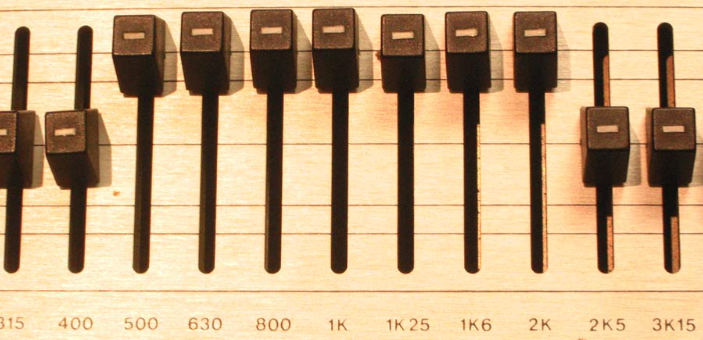
\includegraphics[width=0.6\textwidth]{analog_equalizer}
  \caption{The photo shows an example of an analog equalizer \citep{nordic}.}
  \label{fig:analog_equalizer}
\end{figure}

One amplified bandpass filter will interfere with the neighbouring filters, thus the frequency response will be different than what can be expected with ideal filters. The following \autoref{fig:analog_equalizer_respond} shows the frequency response of the above analog equalizer \autoref{fig:analog_equalizer}.

\begin{figure} [htbp]
 \centering
  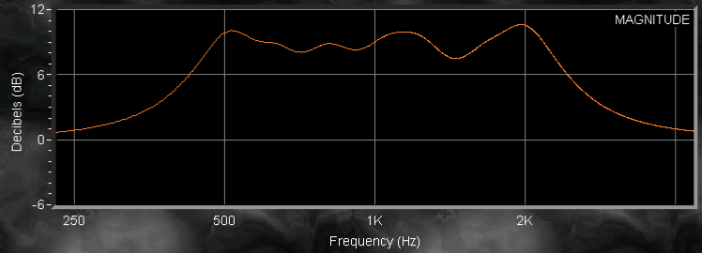
\includegraphics[width=0.8\textwidth]{analog_equalizer_respond}
  \caption{The photo shows the response of the equalizer at \autoref{fig:analog_equalizer} \citep{nordic}.}
  \label{fig:analog_equalizer_respond}
\end{figure}

A simple block diagram of an equalizer is shown in the following \autoref{fig:equalizer_block}.

\begin{figure}[htb] 
	\begin{center} 
\begin{picture}(0,0)%
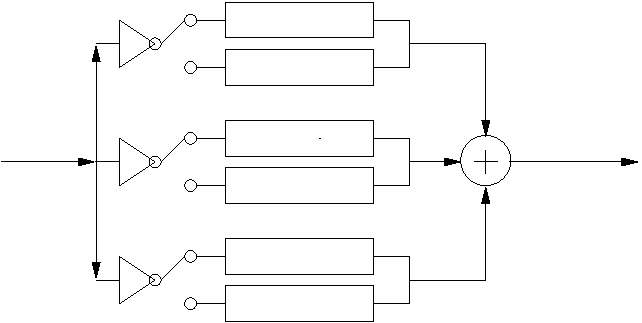
\includegraphics{eq.pdf}%
\end{picture}%
\setlength{\unitlength}{4144sp}%
%
\begingroup\makeatletter\ifx\SetFigFont\undefined%
\gdef\SetFigFont#1#2#3#4#5{%
	\reset@font\fontsize{#1}{#2pt}%
	\fontfamily{#3}\fontseries{#4}\fontshape{#5}%
	\selectfont}%
\fi\endgroup%
\begin{picture}(4884,2454)(3319,-658)
\put(7336,659){\textit{Output}}%

\put(5086,1244){\textit{1st Band}$^{-1}$}%

\put(5086,1604){\textit{1st Band}}%

\put(5086,704){\textit{2nd Band}}%

\put(5131,-196){\textit{3rd Band}}%

\put(5131,-556){\textit{3rd Band}$^{-1}$}%

\put(5086,344){\textit{2nd Band}$^{-1}$}%

\put(3421,749){\textit{Input}}%

\end{picture}%



			\caption{This figure shows a simple block diagram over a equalizer} \label{fig:equalizer_block} 
			\end{center}
			\end{figure}


The block diagram \autoref{fig:equalizer_block} shows a simple equalizer, where the equalizer is divided into separate bandpass filter blocks. Each block is separated by octaves, where the next higher bandpass filter frequency is raised by a factor two. 

